% === [ Results ] ==============================================================

\section{Results}

This section details the results of the control flow recovery methods, when applied to the test programs outlined in section \ref{sec:criteria_for_selection_of_test_programs}. To provide an overview, the results presented are based on the combined test programs of Coreutils and SQLite (individual results of Coreutils and SQLite test programs are presented in appendix \ref{app:coreutils_test_programs} and \ref{app:sqlite_test_programs}, respectively).

Note, due to time constraints in the project, the author has decided to focus on implementing and integrating two out of the three control flow recovery methods with the test suite. Thus, the results present include the results of the Hammock method and the Interval method, but does not include the results of the Pattern-independent method. To help assess the effectiveness of the reviewed methods, they are compared against the theoretical optimum, as further described in section \ref{sec:interpretation_of_results}.

\subsection{Interpretation of Results}
\label{sec:interpretation_of_results}

The results are to be interpreted as follows (previously described in section \ref{sec:project_thesis}).

\begin{itemize}
	\item \textbf{true positive}: control flow primitive \textit{recovered} and \textit{present} in the original source code.
	\item \textbf{false positive}: control flow primitive \textit{recovered} but \textit{not present} in the original source code.
	\item \textbf{false negative}: control flow primitive \textit{present} in the original source code but \textit{not recovered}.
\end{itemize}

In the context of evaluation of effective control flow recovery, \textit{true positive} results are good while both \textit{false positive} and \textit{false negative} results are bad. Extensions to these evaluation metrics are discussed in section \ref{sec:extensions_to_evaluation_metric}.

To provide further perspective, the results of each control flow recovery method are presented along-side the theoretical optimum. The \textit{theoretical optimum} control flow recovery is that all control flow primitives present in the original source code are recovered with correct types (i.e. \textit{true positives}) and that no control flow primitives not present in the original source code are recovered (i.e. \textit{false positives}). Note, by definition, this means that for each control flow primitive type the theoretical optimum has 0 \textit{false negatives}, 0 \textit{false positives} and exactly as many \textit{true positives} as there are control flow primitives of the specific type in the original source code.

% === [ Subsections ] ==========================================================

% --- [ Combined Results ] -----------------------------------------------------

\subsection{Combined Results}
\label{sec:combined_results}

The \textit{combined} control flow recovery results of the Hammock method, the Interval method, and for comparison the theoretical optimum when recovering \textit{2-way conditionals}, \textit{n-way conditionals}, \textit{pre-test loops} and \textit{post-test loops} from the combined test programs of Coreutils and SQLite are presented in figure \ref{fig:total_results_combined}.

The \textbf{Hammock method} correctly recovered $42.16\%$ of the control flow primitives present in the test programs (\textit{true positives}). On average, for every $10$ control flow primitives of the original source code, the Hammock method recovered $3.5$ control flow primitives that were \textit{not} present of the original source code (\textit{false positives}).

The \textbf{Interval method} correctly recovered $74.28\%$ of the control flow primitives present in the test programs (\textit{true positives}). On average, for every $10$ control flow primitives of the original source code, the Interval method recovered $5.9$ control flow primitives that were \textit{not} present of the original source code (\textit{false positives}).

\begin{figure}[htbp]
	\centering
	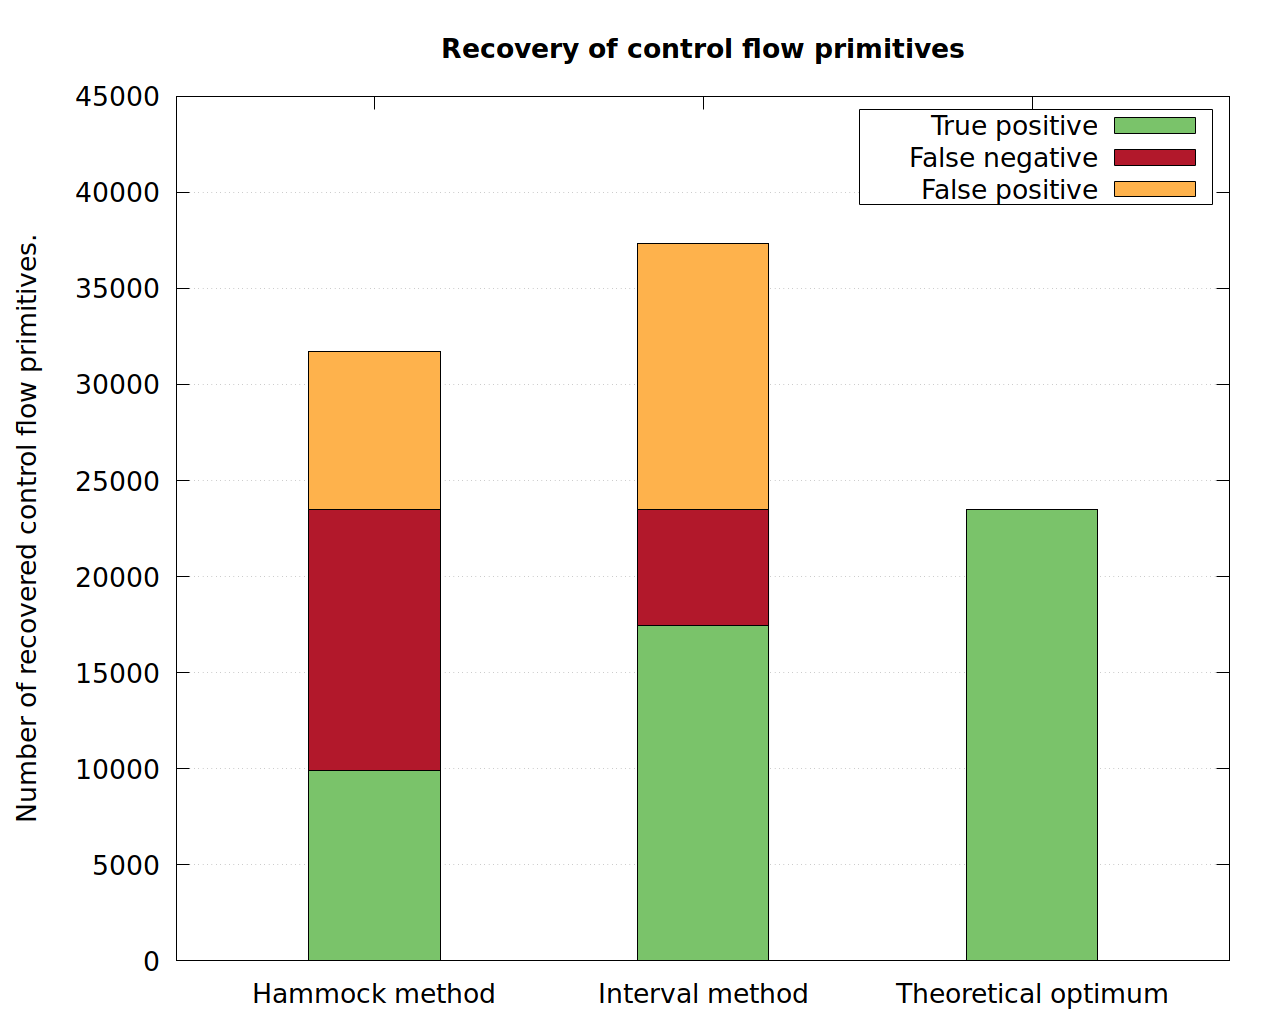
\includegraphics[width=\textwidth]{inc/5_results/results_combined.png}
	\caption{Comparison of control flow recovery results for each method, with the combined results of recovering \textit{2-way conditionals}, \textit{n-way conditionals}, \textit{pre-test loops} and \textit{post-test loops}. The data is based on the combined test programs of Coreutils and SQLite.}
	\label{fig:total_results_combined}
\end{figure}

% --- [ Recovery of 2-way Conditionals ] ---------------------------------------

\subsection{Recovery of 2-way Conditionals}
\label{sec:recovery_of_2way_conditionals}

The control flow recovery results of the Hammock method, the Interval method, and for comparison the theoretical optimum when recovering \textit{2-way conditionals} (e.g. \texttt{if-else} statements) from the combined test programs of Coreutils and SQLite are presented in figure \ref{fig:total_results_2way}.

The \textbf{Hammock method} correctly recovered $46.68\%$ of the 2-way conditionals present in the test programs (\textit{true positives}). On average, for every $10$ 2-way conditionals of the original source code, the Hammock method recovered $3.9$ 2-way conditionals that were \textit{not} present of the original source code (\textit{false positives}).

The \textbf{Interval method} correctly recovered $74.84\%$ of the 2-way conditionals present in the test programs (\textit{true positives}). On average, for every $10$ 2-way conditionals of the original source code, the Interval method recovered $5.0$ 2-way conditionals that were \textit{not} present of the original source code (\textit{false positives}).

Note, at this level of comparison, \textit{if-statements} and \textit{if-else} statements are both regarded as 2-way conditionals. While the Hammock method distinguish 1-way conditionals from 2-way conditionals at the control flow recover stage, the Interval method distinguish 1-way conditionals from 2-way conditionals at the code generation state. For this reason, no distinction is made between 1-way and 2-way conditionals during the evaluation.

\begin{figure}[htbp]
	\centering
	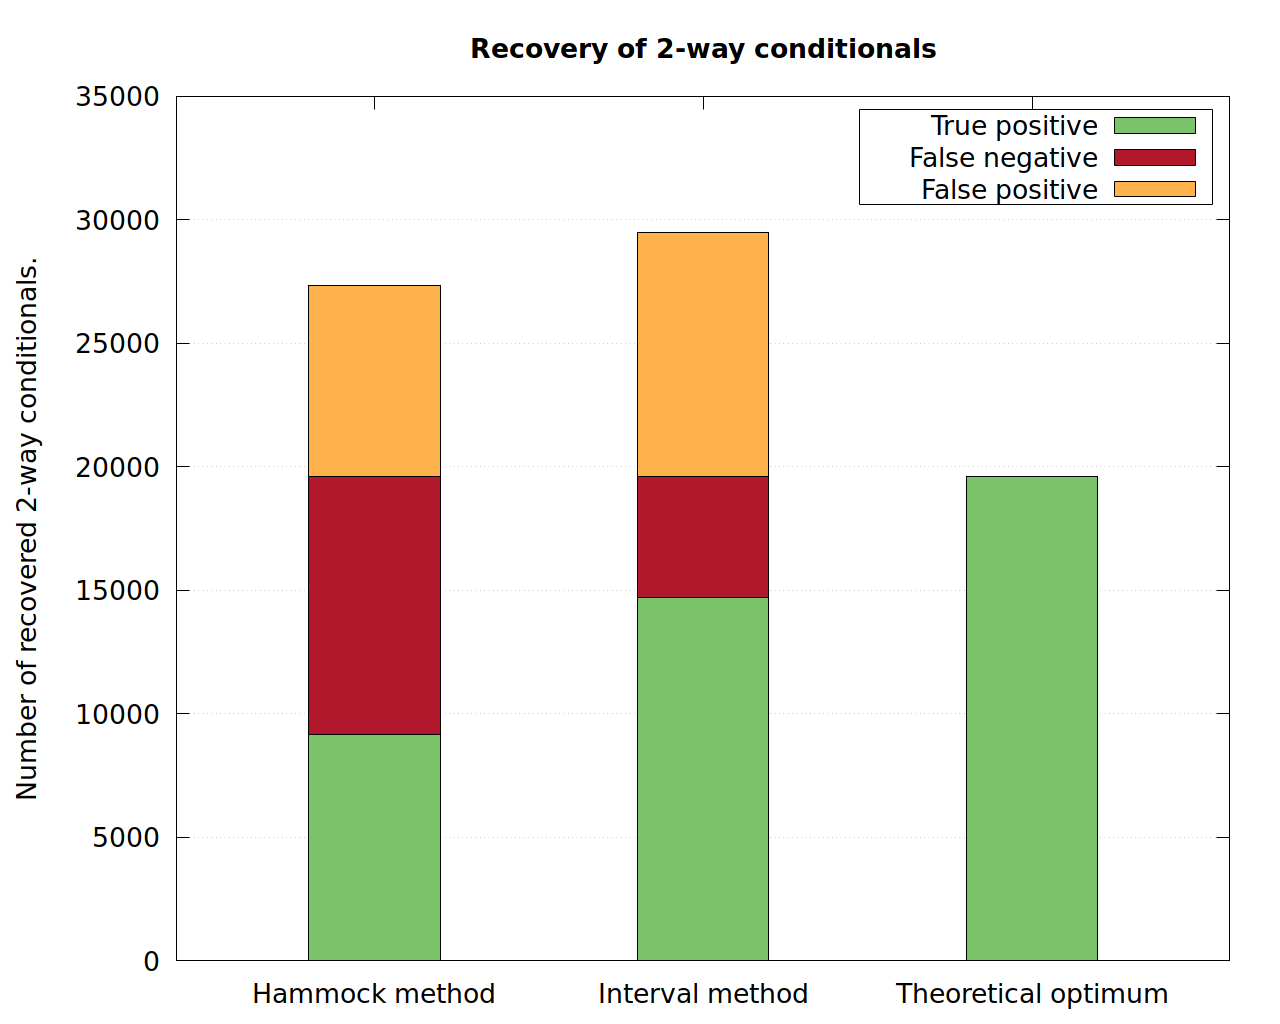
\includegraphics[width=\textwidth]{inc/5_results/results_2-way.png}
	\caption{Comparison of control flow recovery results for each method when recovering \textit{2-way conditionals}. The data is based on the combined test programs of Coreutils and SQLite.}
	\label{fig:total_results_2way}
\end{figure}

% --- [ Recovery of N-way Conditionals ] ---------------------------------------

\subsection{Recovery of N-way Conditionals}
\label{sec:recovery_of_nway_conditionals}

The control flow recovery results of the Hammock method, the Interval method, and for comparison the theoretical optimum when recovering \textit{n-way conditionals} (e.g. \texttt{switch}-statements) from the combined test programs of Coreutils and SQLite are presented in figure \ref{fig:total_results_nway}.

The \textbf{Hammock method} correctly recovered $0.00\%$ of the n-way conditionals present in the test programs (\textit{true positives}). On average, for every $10$ n-way conditionals of the original source code, the Hammock method recovered $3.9$ n-way conditionals that were \textit{not} present of the original source code (\textit{false positives}).

The \textbf{Interval method} correctly recovered $73.40\%$ of the n-way conditionals present in the test programs (\textit{true positives}). On average, for every $10$ n-way conditionals of the original source code, the Interval method recovered $19.7$ n-way conditionals that were \textit{not} present of the original source code (\textit{false positives}).

\begin{figure}[htbp]
	\centering
	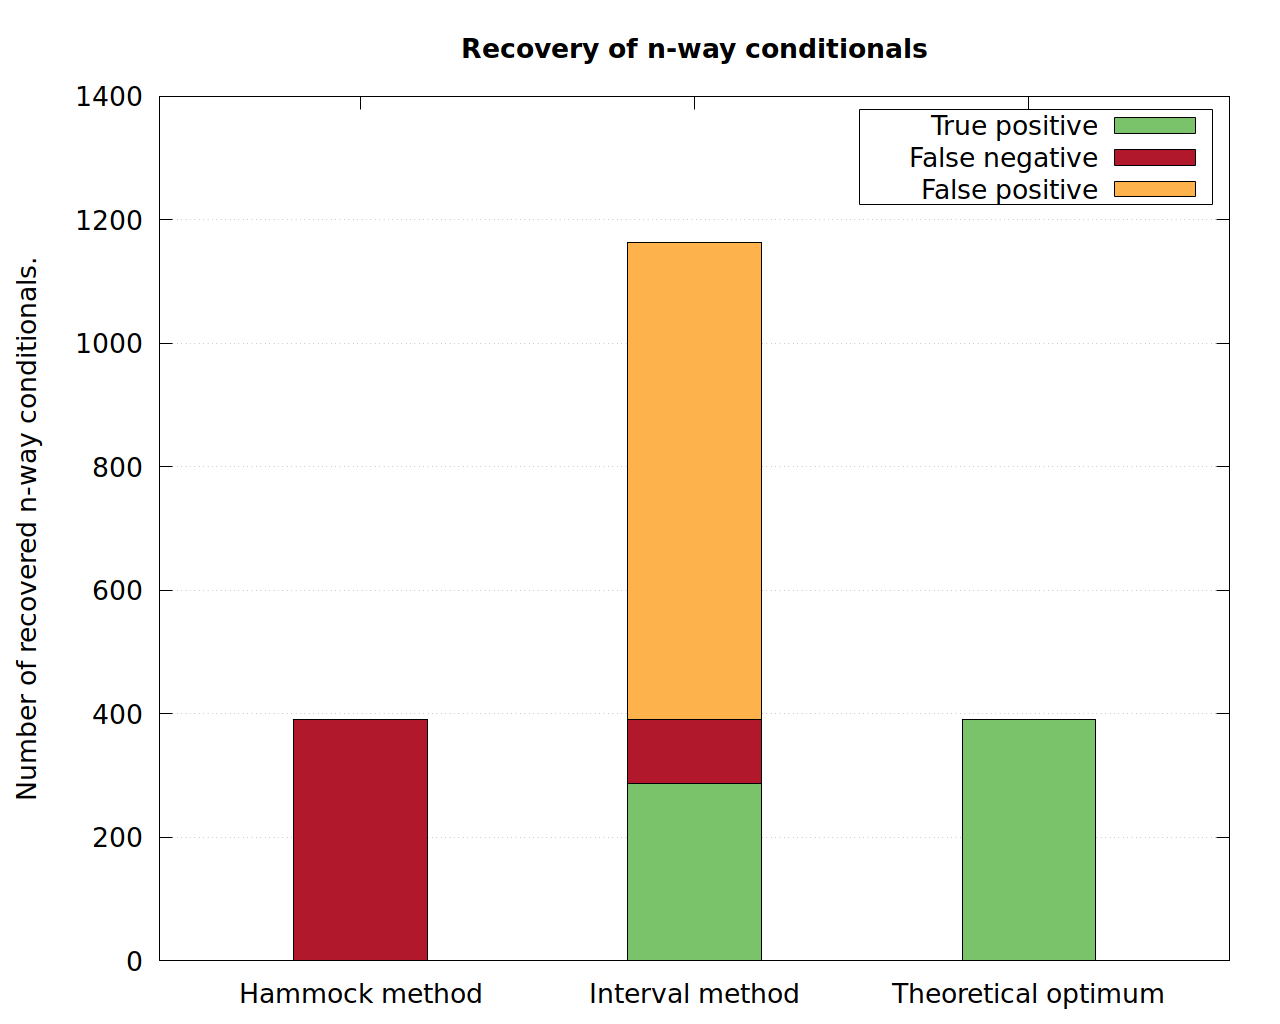
\includegraphics[width=\textwidth]{inc/5_results/results_n-way.png}
	\caption{Comparison of control flow recovery results for each method when recovering \textit{n-way conditionals}. The data is based on the combined test programs of Coreutils and SQLite.}
	\label{fig:total_results_nway}
\end{figure}

% --- [ Recovery of Pre-test Loops ] -------------------------------------------

\subsection{Recovery of Pre-test Loops}
\label{sec:recovery_of_pre_test_loops}

The control flow recovery results of the Hammock method, the Interval method, and for comparison the theoretical optimum when recovering \textit{pre-test loops} (e.g. \texttt{for}-loops) from the combined test programs of Coreutils and SQLite are presented in figure \ref{fig:total_results_pre_loop}.

The \textbf{Hammock method} correctly recovered $29.09\%$ of the pre-test loops present in the test programs (\textit{true positives}). On average, for every $10$ pre-test loops of the original source code, the Hammock method recovered $0.1$ pre-test loops that were \textit{not} present of the original source code (\textit{false positives}).

The \textbf{Interval method} correctly recovered $75.07\%$ of the pre-test loops present in the test programs (\textit{true positives}). On average, for every $10$ pre-test loops of the original source code, the Interval method recovered $4.7$ pre-test loops that were \textit{not} present of the original source code (\textit{false positives}).

Note, at this level of comparison, \textit{pre-test loops} and \textit{infinite loops} are both regarded as pre-test loops. Both the Hammock method and the Interval method distinguish pre-test loops from infinite loops. However, the C parsing script described in step \ref{itm:step_c_to_json} of section \ref{sec:evaluation_process} does not evaluate loop conditions, and can therefore not conclusively determine which conditions are always true (e.g. \texttt{while (TRUE)}). For this reason, no distinction is made between pre-test loops and infinite loops during the evaluation.

\begin{figure}[htbp]
	\centering
	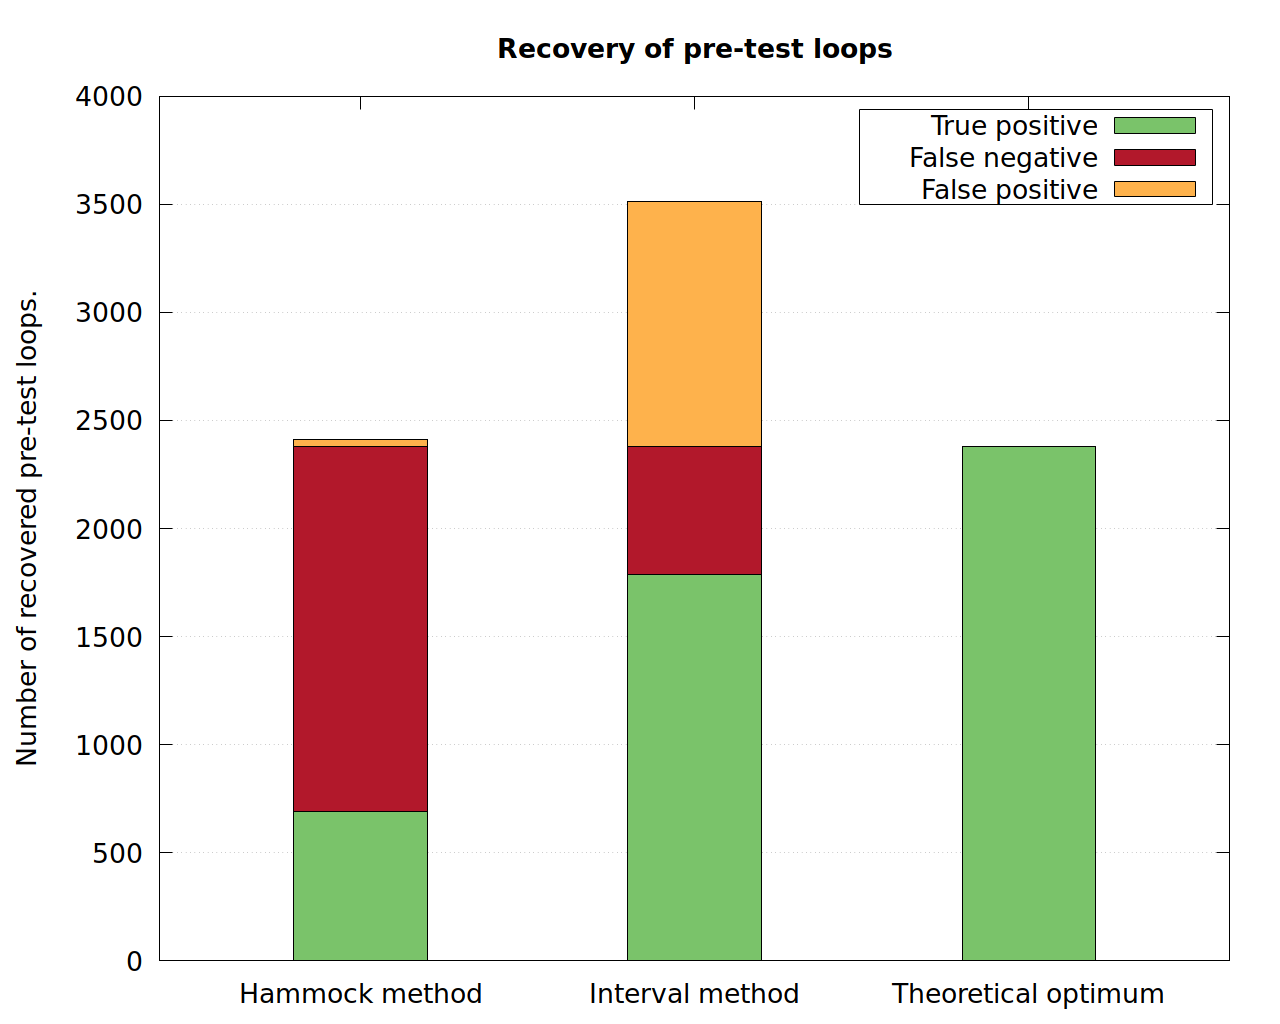
\includegraphics[width=\textwidth]{inc/5_results/results_pre_loop.png}
	\caption{Comparison of control flow recovery results for each method when recovering \textit{pre-test loops}. The data is based on the combined test programs of Coreutils and SQLite.}
	\label{fig:total_results_pre_loop}
\end{figure}

% --- [ Recovery of Post-test Loops ] ------------------------------------------

\subsection{Recovery of Post-test Loops}
\label{sec:recovery_of_post_test_loops}

The control flow recovery results of the Hammock method, the Interval method, and for comparison the theoretical optimum when recovering \textit{post-test loops} (e.g. \texttt{do-while}-loops) from the combined test programs of Coreutils and SQLite are presented in figure \ref{fig:total_results_post_loop}.

The \textbf{Hammock method} correctly recovered $4.65\%$ of the post-test loops present in the test programs (\textit{true positives}). On average, for every $10$ post-test loops of the original source code, the Hammock method recovered $4.1$ post-test loops that were \textit{not} present of the original source code (\textit{false positives}).

The \textbf{Interval method} correctly recovered $62.77\%$ of the post-test loops present in the test programs (\textit{true positives}). On average, for every $10$ post-test loops of the original source code, the Interval method recovered $18.7$ post-test loops that were \textit{not} present of the original source code (\textit{false positives}).

\begin{figure}[htbp]
	\centering
	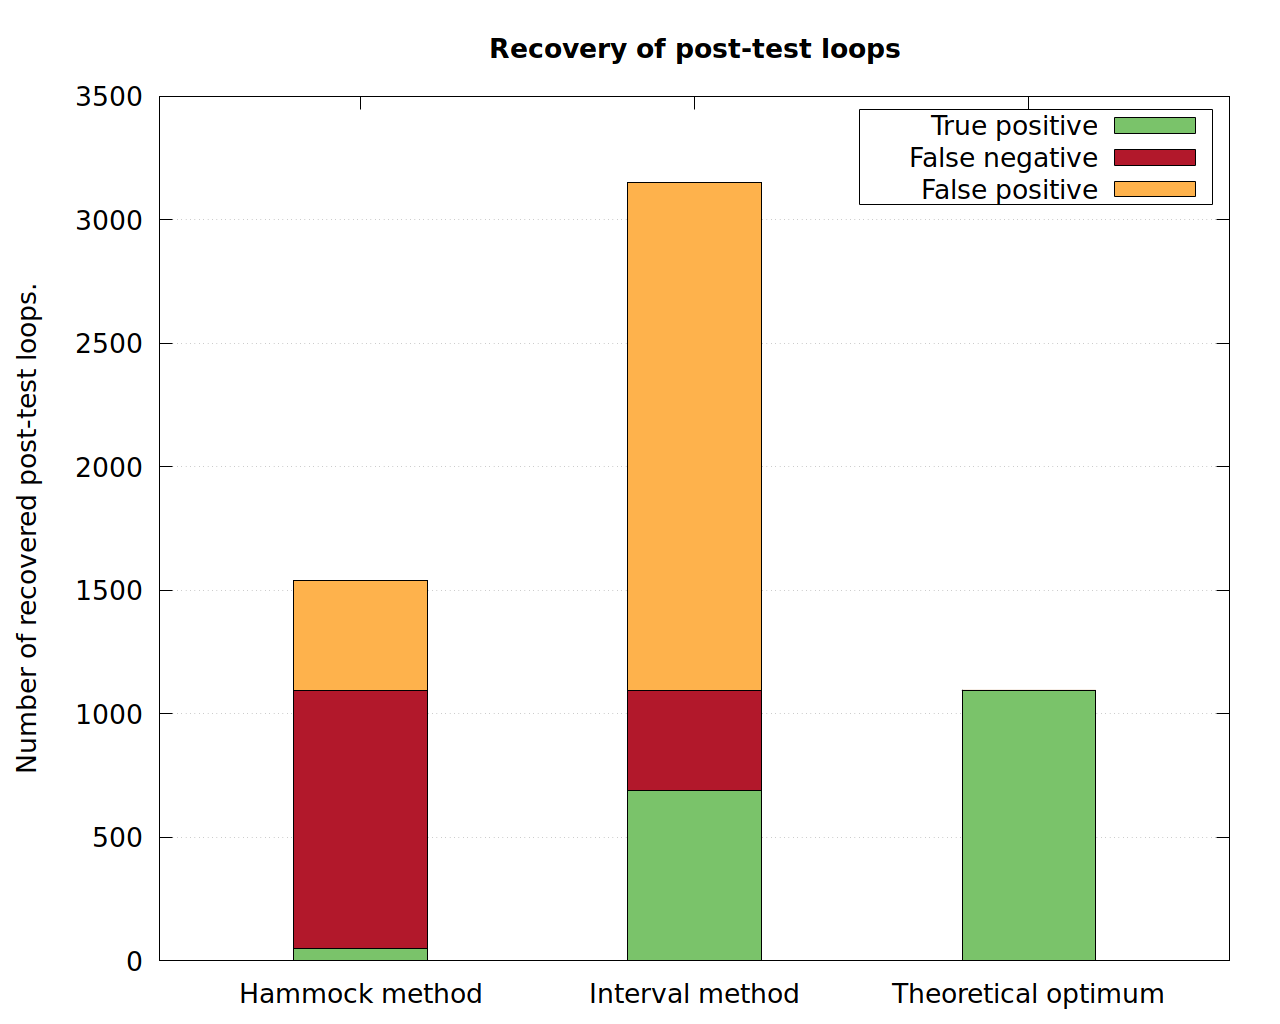
\includegraphics[width=\textwidth]{inc/5_results/results_post_loop.png}
	\caption{Comparison of control flow recovery results for each method when recovering \textit{post-test loops}. The data is based on the combined test programs of Coreutils and SQLite.}
	\label{fig:total_results_post_loop}
\end{figure}

